% Copyright (C) 2014-2023 by Thomas Auzinger <thomas@auzinger.name>

% TODO: remove draft
\documentclass[draft,final]{vutinfth} % Remove option 'final' to obtain debug information.

% Load packages to allow in- and output of non-ASCII characters.
\usepackage{lmodern}        % Use an extension of the original Computer Modern font to minimize the use of bitmapped letters.
\usepackage[T1]{fontenc}    % Determines font encoding of the output. Font packages have to be included before this line.
\usepackage[utf8]{inputenc} % Determines encoding of the input. All input files have to use UTF8 encoding.

% Extended LaTeX functionality is enables by including packages with \usepackage{...}.
\usepackage{amsmath}    % Extended typesetting of mathematical expression.
\usepackage{amssymb}    % Provides a multitude of mathematical symbols.
\usepackage{mathtools}  % Further extensions of mathematical typesetting.
\usepackage{microtype}  % Small-scale typographic enhancements.
\usepackage[inline]{enumitem} % User control over the layout of lists (itemize, enumerate, description).
\usepackage{multirow}   % Allows table elements to span several rows.
\usepackage{booktabs}   % Improves the typesetting of tables.
\usepackage{subcaption} % Allows the use of subfigures and enables their referencing.
\usepackage[ruled,linesnumbered,algochapter]{algorithm2e} % Enables the writing of pseudo code.
\usepackage[usenames,dvipsnames,table]{xcolor} % Allows the definition and use of colors. This package has to be included before tikz.
\usepackage{nag}       % Issues warnings when best practices in writing LaTeX documents are violated.
\usepackage{todonotes} % Provides tooltip-like todo notes.
\usepackage{hyperref}  % Enables hyperlinking in the electronic document version. This package has to be included second to last.
\usepackage[acronym,toc]{glossaries} % Enables the generation of glossaries and lists of acronyms. This package has to be included last.

% custom packages
\usepackage{threeparttable}
\usepackage{makecell}
\usepackage{amsthm}
\usepackage{tikz}
\usetikzlibrary{arrows.meta}

\newtheorem{theorem}{Theorem}
\newtheorem{definition}{Definition}

% Define convenience functions to use the author name and the thesis title in the PDF document properties.
\newcommand{\authorname}{Othmar Lechner} % The author name without titles.
\newcommand{\thesistitle}{T-RACE: Tracing race condition attacks between Ethereum transactions.} % The title of the thesis. The English version should be used, if it exists.

% Set PDF document properties
\hypersetup{
    pdfpagelayout   = TwoPageRight,           % How the document is shown in PDF viewers (optional).
    linkbordercolor = {Melon},                % The color of the borders of boxes around hyperlinks (optional).
    pdfauthor       = {\authorname},          % The author's name in the document properties (optional).
    pdftitle        = {\thesistitle},         % The document's title in the document properties (optional).
    pdfsubject      = {Subject},              % The document's subject in the document properties (optional).
    pdfkeywords     = {a, list, of, keywords} % The document's keywords in the document properties (optional).
}

\setpnumwidth{2.5em}        % Avoid overfull hboxes in the table of contents (see memoir manual).
\setsecnumdepth{subsection} % Enumerate subsections.

\nonzeroparskip             % Create space between paragraphs (optional).
\setlength{\parindent}{0pt} % Remove paragraph indentation (optional).

\makeindex      % Use an optional index.
\makeglossaries % Use an optional glossary.
%\glstocfalse   % Remove the glossaries from the table of contents.

% Set persons with 4 arguments:
%  {title before name}{name}{title after name}{gender}
%  where both titles are optional (i.e. can be given as empty brackets {}).
\setauthor{}{\authorname}{}{male}
\setadvisor{Ass.Prof.in Dipl.-Ing.in Mag.a rer.soc.oec. Dr.in techn.}{Monika di Angelo}{}{female}

% For bachelor and master theses:
\setfirstassistant{Ao.Univ.Prof. Dr.}{Gernot Salzer}{}{male}
% \setsecondassistant{Pretitle}{Forename Surname}{Posttitle}{male}
% \setthirdassistant{Pretitle}{Forename Surname}{Posttitle}{male}

% For dissertations:
% \setfirstreviewer{Pretitle}{Forename Surname}{Posttitle}{male}
% \setsecondreviewer{Pretitle}{Forename Surname}{Posttitle}{male}

% For dissertations at the PhD School and optionally for dissertations:
% \setsecondadvisor{Ao.Univ.Prof. Dipl.-Ing. Dr.techn.}{Gernot Salzer}{}{male} % Comment to remove.

% Required data.
\setregnumber{11841833}
\setdate{01}{01}{2001} % Set date with 3 arguments: {day}{month}{year}.
\settitle{\thesistitle}{T-RACE: Eine Analyse von race condition Angriffen bei Ethereum Transaktionen} % Sets English and German version of the title (both can be English or German). If your title contains commas, enclose it with additional curvy brackets (i.e., {{your title}}) or define it as a macro as done with \thesistitle.
% \setsubtitle{Optional Subtitle of the Thesis}{Optionaler Untertitel der Arbeit} % Sets English and German version of the subtitle (both can be English or German).

% Select the thesis type: bachelor / master / doctor.
% Bachelor:
% \setthesis{bachelor}
%
% Master:
\setthesis{master}
% TODO: dipl. or master?
\setmasterdegree{dipl.} % dipl. / rer.nat. / rer.soc.oec. / master
%
% Doctor:
%\setthesis{doctor}
%\setdoctordegree{rer.soc.oec.}% rer.nat. / techn. / rer.soc.oec.

% For bachelor and master:
\setcurriculum{Software Engineering \& Internet Computing}{Software Engineering \& Internet Computing} % Sets the English and German name of the curriculum.

% Optional reviewer data:
\setfirstreviewerdata{Affiliation, Country}
\setsecondreviewerdata{Affiliation, Country}


\begin{document}

\frontmatter % Switches to roman numbering.
% The structure of the thesis has to conform to the guidelines at
%  https://informatics.tuwien.ac.at/study-services

\addtitlepage{naustrian} % German title page.
\addtitlepage{english} % English title page.
\addstatementpage

\begin{danksagung*}
    \todo{Ihr Text hier.}
\end{danksagung*}

\begin{acknowledgements*}
    \todo{Enter your text here.}
\end{acknowledgements*}

\begin{kurzfassung}
    \todo{Ihr Text hier.}
\end{kurzfassung}

\begin{abstract}
    \todo{Enter your text here.}
\end{abstract}

% Select the language of the thesis, e.g., english or naustrian.
\selectlanguage{english}

% Add a table of contents (toc).
\tableofcontents % Starred version, i.e., \tableofcontents*, removes the self-entry.

% Switch to arabic numbering and start the enumeration of chapters in the table of content.
\mainmatter

\chapter{Introduction}
\todo{Enter your text here.}

\iffalse
    \section{Related work}

    Interesting things:
    - name
    - source is available?
    - does it use RPC / instrumentation / native tracing?
    - does it detect some kind of frontrunning

    See table \ref{tab:blockchain_history_analyzers}.


    % TODO: is there related work in the parallel EVM field? TOD is highly relevant for this
    % https://ieeexplore.ieee.org/abstract/document/10102454


    \begin{table}[h]
        \begin{center}
            \begin{tabular}{ | l | c  | c | c | c | }
                \hline
                Tool/Authors                                     & Scope            \\ \hline
                EthScope \cite{wu_time-travel_2022}              & Generalized      \\ \hline
                TokenScope \cite{chen_tokenscope_2019}           & ERC-20 tokens    \\ \hline
                TXSPECTOR \cite{zhang_txspector_2020}            & Generalized      \\ \hline
                Horus \cite{ferreira_torres_eye_2021}            & Generalized      \\ \hline
                SODA \cite{chen_soda_2020}                       & Generalized      \\ \hline
                DEFIER \cite{su_evil_2021}                       & Generalized      \\ \hline
                Zhou et al. \cite{zhou_ever-evolving_2020}       & Generalized      \\ \hline
                Perez et al. \cite{perez_smart_2021}             & Generalized      \\ \hline
                Wang et al. \cite{wang_impact_2022}              & Sandwich attacks \\ \hline
                Erebus-redgiant \cite{zhang_combatting_2023}     & Frontrunning     \\ \hline
                Frontrunner Jones \cite{torres_frontrunner_2021} & Frontrunning     \\ \hline
            \end{tabular}
            \caption{Blockchain history analysis references. Generalized means, that the data collection and analysis framework is not tailored to specific vulnerabilities.}
            \label{tab:blockchain_history_analyzers}
        \end{center}
    \end{table}
    \todo{Better caption}

    \section{Related approaches}

    \subsection{Combatting paper - Erebus-redgiant}

    How do they replay potential attack/victim transactions?

    Their framework allows forking at a specific block and tx index.

    PrepareStateAndContext - replays up to tx index.


    They skip potential victim transactions if:

    \begin{enumerate}
        \item error victim transactions (\todo{Are these failed transactions in Ethereum, or error somewhere in their framework? If it's the first, why???})
        \item "filtered" transactions \todo{What are these?}
        \item unverified contracts in victim transactions
        \item victim tx is contract creation (why???). But a good label :)
        \item victim tx is ether transfer
        \item no overlap with attack tx (compare sets of contracts/accounts)
        \item no dependency (storage and balance dependencies, but seem to ignore dependencies within reverted calls)
    \end{enumerate}

    Replaying in the attack free scenario:

    \begin{enumerate}
        \item take attack tx state (I guess prestate)
        \item take victim context (I guess block environment, timestamp, ...)
        \item apply "prerequesites" - all previous transactions from the same sender within (attack, victim-1)?
        \item apply + trace victim tx
        \item apply + trace attack tx
    \end{enumerate}

    For prerequisites, refer to \href{https://github.com/Troublor/erebus-redgiant/blob/4544163f0c6a369b35c3237851f482d240fa7bbd/dataset/tx_history_test.go#L42-L53}.

    Problems with this approach:

    \begin{enumerate}
        \item Prerequisites is an arbitrary choice
              \subitem what if prerequisites have collisions with the attack?
              \subitem what if prerequisites depend on other transactions that were not replayed?
              \subitem what if victim tx depends on other transactions that were not replayed?
        \item all transactions share the same context
              \subitem attack tx is moved to different context
              \subitem prerequisites are potentially moved to different context
              \subitem (victim tx stays in same context \checkmark)
        \item replay is done with a different environment
    \end{enumerate}
\fi

\section{Contributions}

\begin{itemize}
    \item Precise definition of TOD in the context of blockchain transaction analysis.
    \item Theoretical discussion of TOD, including compilation of instructions that can cause TOD.
    \item Methodology to mine potential TOD transaction pairs using only the RPC interface of an archive node, rather than directly accessing it.
\end{itemize}

\chapter{Background}

This chapter gives background knowledge on Ethereum, that is helpful to follow the remaining paper.

\section{Ethereum}

Ethereum is a blockchain, that can be characterized as a "transactional singleton machine with shared-state" \cite{wood_ethereum_2024}. By using a consensus protocol, a decentralized set of nodes agrees on a globally shared state. This state contains two types of accounts: \emph{externally owned accounts} (EOA) and \emph{contract accounts} (also referred to as smart contracts). Each account is identified by a 20 byte address. The shared state is modified by executing \emph{transactions} \cite{tikhomirov_ethereum_2018}.

\section{World State}

Similar to \cite{wood_ethereum_2024}, we will refer to the shared state as \emph{world state}. The world state maps addresses to account states, containing a \emph{nonce}, \emph{balance}, \emph{storage} and \emph{code}\footnote{Technically, the account state only contains hashes that identify the storage and code, not the actual storage and code. This distinction is not relevant in this paper.}. They store following data \cite{wood_ethereum_2024}:

\begin{itemize}
    \item \emph{nonce}: For EOAs, this is the number of transactions submitted by this account. For contract accounts, this is the number of contracts created by this account.
    \item \emph{balance}: The value of Wei, a smaller unit of Ether.
    \item \emph{storage}: For contract accounts, the storage a mapping of storage slots to values. Both, key and value, are 256 bytes. For EOAs, this is empty.
    \item \emph{code}: For contract accounts, the code is a sequence of EVM instructions.
\end{itemize}

We denote the world state as $\sigma$, the account state of an address $a$ as $\sigma(a)$ and the nonce, balance, storage and code as $\sigma(a)_n$, $\sigma(a)_b$, $\sigma(a)_s$ and $\sigma(a)_c$ respectively. For the value at a storage slot $k$ we write $\sigma(a)_s[k]$. We will also an alternative notation $\sigma(K)$ to denote the state value at some state key $K$. Following notations will be used:

\begin{align*}
    \sigma(a)_n    & = \sigma(("nonce", a))      \\
    \sigma(a)_b    & = \sigma(("balance", a))    \\
    \sigma(a)_c    & = \sigma(("code", a))       \\
    \sigma(a)_s[k] & = \sigma(("storage", a, k)) \\
\end{align*}

\section{EVM}

The Ethereum Virtual Machine (EVM) is used to execute code in Ethereum. It can execute a set of instructions, that can access and modify the world state. The EVM is Turing-complete, except that it is executed with a limited amount of \emph{gas} and each instruction costs some gas \cite{wood_ethereum_2024}. When it runs out of gas, the execution will halt \cite[p.14]{wood_ethereum_2024}. For instance, this prevents execution of infinite loops, as it would use infinitely much gas and thus exceed the gas limit.

Most EVM instructions are formally defined in \cite[p.30-38]{wood_ethereum_2024}. However, the Yellowpaper currently does not include the changes from the Cancun upgrade \cite{noauthor_history_2024}, therefore we will also refer to the informal description available on \href{https://www.evm.codes/}{evm.codes} \cite{noauthor_evm_2024}.

\section{Transactions}

A transaction can modify the world state by transferring Ether and executing EVM code. It must be signed by the owner of an EOA and contains following data relevant to our work:

\begin{itemize}
    \item \emph{sender}: The address of the transaction sender\footnote{The sender is only implicitly given through the signature and the transaction hash \cite[p.25-27]{wood_ethereum_2024}. We are only interested in transactions that are included in the blockchain, thus the signature must be valid and the transaction's sender can always be computed.}.
    \item \emph{recipient}: The destination address.
    \item \emph{value}: The value of Wei that should be transferred from the sender to the recipient.
    \item \emph{gasLimit}: The maximum number of gas, that can be used for the execution.
\end{itemize}

If the recipient address is empty, the transaction will create a new contract account. These transactions also include an \emph{init} field, that contains the code to initialize the new contract account.

When the recipient address is given, the value will be transferred to the recipient and, if the recipient is a contract account, also execute the recipient's code. The transaction can specify a \emph{data} field to pass input data to the code execution \cite[p.4-5]{wood_ethereum_2024}.

% TODO: move \cite to pre/post period.

For every transaction the sender must pay a \emph{transaction fee}. This is composed of a \emph{base fee} and a \emph{priority fee}. Every transaction must pay the base fee. The amount of Wei will be reduced from the sender and not given to any other account. For the priority fee, the transaction can specify if, and how much they are willing to pay. This fee will be taken from the sender and given to the block validator, explained in the next section \cite[p.8]{wood_ethereum_2024}.

We denote a transaction as $T$, sometimes adding a subscript $T_A$ to differentiate from another transaction $T_B$.

% TODO: rename block producer to block validator

\section{Blocks}

The Ethereum blockchain consists of a sequence of blocks, where each block builds upon the state of the previous block. To achieve consensus about the canonical sequence of blocks in a decentralized network of nodes, Ethereum currently uses a consensus protocol. In this protocol, validators build and propose blocks to be added to the blockchain \cite{noauthor_gasper_2024}. It is the choice of the validator, which transactions to include in a block, however they are incentivized to include transactions that pay high transaction fees, as they receive the fee \cite[p.8]{wood_ethereum_2024}.

Each block consists of a block header and a sequence of transactions. We denote the nth block of the blockchain as $B_n$ and the sequence of transactions it includes as $T(B_n) = (T_1, T_2, \dots, T_m)$.

\section{Transaction submission}

This section discusses, how a signed transaction by an EOA ends up being included in the blockchain.

Traditionally, the signed transaction is broadcasted to the network of nodes, which temporarily store them in a \emph{mempool}, a collection of pending transactions. The creator of the next block then picks transactions from the mempool and includes them in the next block \cite{eskandari_sok_2020}. In this submission method, the pending transactions in the mempool are publicly known to the nodes in the network, even before being included in the blockchain. This time window will be important for our discussion on frontrunning, as it gives nodes time to react on a transaction before it is executed on the blockchain.

A different approach, the Proposer-Builder Separation (PBS) has become more popularity recently: Here, we separate the task of collecting transactions and building blocks with them from the task of proposing them as a validator \cite{heimbach_ethereums_2023}. A user submits their signed transaction or transaction bundle to a block builder. The block builder has a private mempool and uses it to create profitable blocks. Finally, the validator picks one of the created blocks and adds it to the blockchain.

\section{Transaction execution}

In Ethereum, transaction execution is deterministic: If the transaction is executed in a specific block environment and world state, it will always produce the same result\todo{Reference}. The result is used to update the world state.

In this paper, we are interested in the effects of the transaction order. If we reorder transactions across multiple blocks, they would execute in a different block environment than they did originally. The effects of different block environments are already covered in several other vulnerability definitions\todo{Reference}. In this work, we will exclude the possibility of changing block environments and assume that transactions are always executed in their original block environment.

We denote a transaction execution as $\sigma \xrightarrow{T} \sigma\prime$, implicitly letting the block environment correspond to the transaction's block. Furthermore, we denote the \emph{state diff} done by a transaction $T$ as $\Delta_T$, with $prestate(\Delta_T) = \sigma$ being the state before execution and $poststate(\Delta\sigma_T) = \sigma\prime$ the state after the execution of $T$.

For two state changes $\Delta_{T_A}$ and $\Delta_{T_B}$, we say that $\Delta_{T_A} = \Delta_{T_B}$ if they changed the same set of state fields and the pre- and poststate for these changed fields is equal. Otherwise, we say $\Delta_{T_A} \neq \Delta_{T_B}$. For instance, if both $\Delta_{T_A}$ and $\Delta_{T_B}$ modified only the storage $\sigma(a)_s[k]$, and both changed it from the value $x$ to the value $y$, we would call them equal. If $\Delta_{T_B}$ changed it from $x\prime$ to $y$, or from $x$ to $y\prime$ or even modified a different storage slot $\sigma(a)_s[k\prime]$, we would say $\Delta_{T_A} \neq \Delta_{T_B}$.

We define the set of changed state keys as:

$$changed\_keys(\Delta) \coloneqq \{ K | prestate(\Delta)(K) \neq poststate(\Delta)(K) \}$$

We let the equality $\Delta_{T_A} = \Delta_{T_B}$ be true if following holds, else $\Delta_{T_A} \neq \Delta_{T_B}$:

\begin{align*}
    changed\_keys(\Delta_{T_A})       & = changed\_keys(\Delta_{T_B})                           \\
    \forall K \in changed\_keys\colon &
    prestate(\Delta_{T_A})(K) = prestate(\Delta_{T_B})(K)                                       \\
    \text{ and }                      & poststate(\Delta_{T_B})(K) = poststate(\Delta_{T_B})(K)
\end{align*}

We define $\sigma + \Delta_T$ to be equal to the state $\sigma$, except that every state that was changed by the execution of $T$ is overwritten with the value in $poststate(\Delta_T)$. Similarly, $\sigma - \Delta_T$ is equal to the state $\sigma$, except that every state that was changed by the execution of $T$ is overwritten with the value in $prestate(\Delta_T)$. Formally, these definitions are as follows:

\begin{align*}
    (\sigma + \Delta_T)(K) & \coloneqq
    \begin{cases}
        poststate(\Delta_T)(K), & K \in changed\_keys(\Delta_T) \\
        \sigma(K),              & \text{otherwise}
    \end{cases} \\
    (\sigma - \Delta_T)(K) & \coloneqq
    \begin{cases}
        prestate(\Delta_T)(K), & K \in changed\_keys(\Delta_T) \\
        \sigma(K),             & \text{otherwise}
    \end{cases}
\end{align*}

For instance, if transaction $T$ changed the storage slot 1234 at address 0xabcd from 0 to 100, then $(\sigma + \Delta_T)(\text{0xabcd})_s[1234] = 100$ and $(\sigma - \Delta_T)(\text{0xabcd})_s[1234] = 0$. For all other storage slots we have $(\sigma + \Delta_T)(a)_s[k] = \sigma(a)_s[k] = (\sigma - \Delta_T)(a)_s[k]$.

\section{Nodes}

A node consists of an \emph{execution client} and a \emph{consensus client}. The execution client keeps track of the world state and the mempool and executes transactions. The consensus client takes part in the consensus protocol. For this work, we will use an \emph{archive node}, which is a node that allows to reproduce the state and transactions at any block \cite{noauthor_nodes_2024}.

\section{RPC}

Execution clients implement the Ethereum JSON-RPC specification \cite{noauthor_ethereum_2024}. It provides an API to access the execution client, for instance to inspect the current block number with \verb|eth_blockNumber| or to execute a transaction without committing the state via \verb|eth_call|. In addition to the standardized RPC methods, we will also make use of methods in the debug namespace, such as \verb|debug_traceBlockByNumber|. While this namespace is not standardized, several execution clients implement these additional methods \cite{noauthor_debug_2024}\cite{noauthor_rpc_2024}\cite{noauthor_reth_2024}.

\chapter{Transaction order dependency}

In this chapter we discuss our definition of transaction order dependency (TOD) and various properties that come with it. We first lay out the idea of TOD with a basic definition and then show several shortcomings of a simple definition and how this affected previous works. Based on these insights, we construct a more precise definition that we will use for our analysis.

\section{Approaching TOD}

Intuitively, a pair of transactions $(T_A, T_B)$ is transaction order dependent (TOD), if the original execution order leads to a different result than a reordered execution order. In formal terms, we write this as following:

$$\sigma \xrightarrow{T_A, T_B} \sigma \prime$$
$$\sigma \xrightarrow{T_B, T_A} \sigma \prime \prime$$
$$\sigma \prime \neq \sigma \prime \prime$$

So, starting from an initial state, when we execute first $T_A$ and then $T_B$ it will result in a different state, than when executing $T_B$ and afterwards $T_A$.

We will refer to the execution order $T_A \rightarrow T_B$, the one that occurred on the blockchain, as the \emph{normal} execution order, and $T_B \rightarrow T_A$ as the \emph{reversed} execution order.

\section{Motivating examples}

\todo{Add a motivating example for write-read TOD (e.g. TOD-recipient) and for write-write TOD (e.g. ERC-20 approval).}

\section{Relation to previous works}

In \cite{torres_frontrunner_2021} the authors do not provide a formal definition of TOD. However, for displacement attacks, they include the following check to detect if two transactions fall into this category:

\begin{quote}
    [...] we run in a simulated environment first $T_A$ before $T_V$ and then $T_V$ before $T_A$. We report a finding if the number of executed EVM instructions is different across both runs for $T_A$ and $T_V$, as this means that $T_A$ and $T_V$ influence each other.
\end{quote}

Similar to our intuitive TOD definition, they execute $T_A$ and $T_V$ in different orders and check if it affects the result. In their case, they only check the number of executed instruction, instead of the resulting state. This would miss attacks where the same instructions were executed, but the operands for these instructions in the second transaction changed because of the first transaction.

In \cite{zhang_combatting_2023}, they define an attack as a triple $A = \langle T_a, T_v, T_a^p\rangle$, where $T_a$ and $T_v$ are similar to our $T_A$ and $T_B$, and $T_a^p$ is an optional third transaction. With these they model the execution orders $T_a \rightarrow T_v \rightarrow T_a^p$ and $T_v \rightarrow T_a \rightarrow T_a^p$. They then use the results to check if the execution order impacts financial gains, which we will discuss in a later section\todo{Reference section}.

First, we note that if these two execution orders result in different states, this is not because of the last transaction $T_a^p$, but because of a TOD between $T_a$ and $T_v$. If this was not the case, and $T_a \rightarrow T_v$ and $T_v \rightarrow T_a$ would result in the same state but executing $T_a^p$ afterwards would result in two different states, then $T_a^p$ would not be deterministic.

Therefore, if the execution order results in different financial gains, then $T_a$ and $T_v$ must be TOD. Thus, transaction order dependency is a prerequisite for the attacks in \cite{zhang_combatting_2023}.

\section{Imprecise definitions}

Our intuitive definition of TOD, and the related definitions shown above, are not precise on the semantics of an ordering and reordering of transactions and their executions. These make it impossible to apply the same methodology without analyzing the source code related to the papers. We detect three issues, where the definition is not precise enough and was interpreted differently by the two papers.

For the analysis of the tools by \cite{zhang_combatting_2023} and \cite{torres_frontrunner_2021}, we will use the current version of the source codes, \cite{noauthor_troublorerebus-redgiant_2024} and \cite{noauthor_christoftorresfrontrunner-jones_2024} respectively.

\subsection{Intermediate transactions}

To analyze the TOD $(T_A, T_B)$, we are interested in how $T_A$ affected $T_B$. For now, we did not specify how we handle transactions that occurred between $T_A$ and $T_B$.

For instance, let us assume that there was one transaction $T_X$ in between $T_A$ and $T_B$: $\sigma \xrightarrow{T_A} \sigma_A \xrightarrow{T_X} \sigma_{AX} \xrightarrow{T_B} \sigma_{AXB}$. As such, the execution of $T_B$ could depend on both $T_A$ and $T_X$.

For executing the normal order, we would have two possibilities:

\begin{enumerate}
    \item $\sigma \xrightarrow{T_A} \sigma_A \xrightarrow{T_B} \sigma_{AB}$, and thus having a normal execution that potentially diverges from the results on the blockchain (as $\sigma_{AB}$ may differ to $\sigma_{AXB}$).
    \item $\sigma \xrightarrow{T_A} \sigma_A \xrightarrow{T_X} \sigma_{AX} \xrightarrow{T_B} \sigma_{AXB}$, the same execution as on the blockchain, including the effects of $T_X$.
\end{enumerate}

When executing the reverse order, we could make following choices:

\begin{enumerate}
    \item $\sigma \xrightarrow{T_B} \sigma_B \xrightarrow{T_A} \sigma_{BA}$, which ignores $T_X$ and thus may impact the execution of $T_B$.
    \item $\sigma \xrightarrow{T_X} \sigma_X \xrightarrow{T_B} \sigma_{XB} \xrightarrow{T_A} \sigma_{XBA}$, which executes $T_X$  on $\sigma$ rather than $\sigma_A$, which was originally used for $T_X$.
\end{enumerate}

\todo{What about logs? These are not part of the world state, but could/should also be modelled. On the other hand, a TOD log without a TOD resulting state seems unlikely / like a useless log in the first place.}

All of these scenarios are possible, but none of them provides a clean solution to solely analyze the impact of $T_A$ on $T_B$, as we always could have some indirect impact from the (non-)execution of $T_X$.

In \cite{zhang_combatting_2023}, this impact of the intermediary transactions is acknowledged and caused a few false positives:

\begin{quote}
    In blockchain history, there could be many other transactions between $T_a$, $T_v$, and $T_p^a$. When we change the transaction orders to mimic attack-free scenarios, the relative orders between $T_a$ (or $T_v$) and other transactions are also changed. Financial profits of the attack or victim could be affected by such relative orders. As a result, the financial profits in the attack-free scenario could be incorrectly calculated, and false-positively reported attacks may be induced, but our manual check shows that such cases are rare.
\end{quote}

Nonetheless, it is not clear, which of the above scenarios they applied for their analysis. \cite{torres_frontrunner_2021} does not mention this issue at all.

\todo{Should I move the technical aspects to an appendix?}

\subsubsection{Analysis of \cite{zhang_combatting_2023}}


As shown in their algorithm 1, they take as input all the executed transactions. They use these transactions and their results in the \verb|searchVictimGivenAttack| method, where \verb|ar| represents the attack transaction and result and \verb|vr| represents the victim transaction and result.

For the normal execution order, they simply use \verb|ar| and \verb|vr| and pass them to their \verb|CheckOracle| method which then compares the resulting states. As they use the results obtained from executing all transactions, they also include the intermediary transactions for these results (similar to our $\sigma \xrightarrow{T_A} \sigma_A \xrightarrow{T_X} \sigma_{AX} \xrightarrow{T_B} \sigma_{AXB}$ case).

For the reverse order ($T_a \rightarrow T_v$), they take the state before $T_a$, i.e. $\sigma$. Then they execute all transactions obtained from the \verb|SlicePrerequisites| method. And finally they execute $T_v$ and $T_a$.

The \verb|SlicePrerequisites| method uses the \verb|hbGraph| built in \verb|StartSession|, which seems to be a graph where each transaction points to the previous transaction from the same EOA. From this graph, it takes all transactions between $T_a$ and $T_v$, that are from the same sender as $T_v$. This interpretation matches the test case "should slide prerequisites correctly" from the source code. As the paper does not mention these prerequisite transactions, we do not know why this subset of intermediary transactions was chosen.

We can conclude, that for the reverse order, \cite{zhang_combatting_2023} executes all intermediary transactions for the normal order. However, for the reverse order, they only execute intermediary transactions that are also sent by the victim, but do not execute any other intermediary transactions.

\subsubsection{Analysis of \cite{torres_frontrunner_2021}}

In the file \verb|displacement.py|, they replay the normal execution order at the lines 154-155, and the reverse execution order at the lines 158-159 from line 151 to 159. As we can see here, they only execute $T_A$ and $T_V$ (in normal and reverse order), but do not execute any intermediate transactions.

\subsection{Block environments}

When we have a TOD between $T_A$ and $T_B$ it can be, that these are not part of the same block. As transactions can access some data from the block they are in, for instance the block number, the execution of a transaction can depend on the block environment. From our intuitive TOD definition, it is not clear which block environment(s) we use when replaying the transactions in normal and reverse order.

Changing this environment could change the outcome of the transaction. In particular, if we do not use the same block environment as on the blockchain, we may get different results in the analysis than actually happened on the blockchain.

\subsubsection{Analysis of \cite{zhang_combatting_2023}}

The block environment used to execute all transactions is contained in \verb|ar.VmContext| and as such corresponds to the block environment of $T_a$. This means $T_a$ is executed in the same block environment as on the blockchain, while $T_v$ and the intermediary transactions may be executed in a different block environment.

\subsubsection{Analysis of \cite{torres_frontrunner_2021}}

In the file \verb|displacement.py| line 151, we see that the emulator uses the same block environment for both transactions. Therefore, at least one of them will be executed in a different block environment than on the blockchain.

\subsection{Initial state $\sigma$}

While our preliminary TOD definition specifies that we start with the same $\sigma$ in both execution orders, it is up to interpretation which world state $\sigma$ is.

\subsubsection{Analysis of \cite{zhang_combatting_2023}}

The initial state used to execute the first transaction is \verb|ar.State|, which corresponds to the state directly before executing $T_a$. This includes all previous transactions of the same block.

\subsubsection{Analysis of \cite{torres_frontrunner_2021}}

The emulator is initialized with the block \verb|front_runner["blockNumber"]-1|. They do not modify the emulator before executing the transactions, thus $\sigma$ must directly be derived from the block and is the state after executing a whole block. As the emulator does not include state changes from a subset of transactions from a block, it also does not include any transaction that was executed before $T_A$ in the same block.

Similar to the block environment, this could lead to differences in the emulation and the results from the blockchain, if $T_A$ or $T_V$ is impacted by a previous transaction in the same block.

\section{TOD definition}

To address the issues above, we will provide a more precise definition for TOD.

\begin{definition}[TOD]
    Consider a sequence of transactions, with $\sigma$ being the world state right before $T_A$ was executed on the blockchain:

    $$\sigma \xrightarrow{T_A} \sigma_A \xrightarrow{T_{X_1}} \dots \xrightarrow{T_{X_n}} \sigma_{X_n} \xrightarrow{T_B} \sigma_B$$

    Let $\Delta_{T_A}$ and $\Delta_{T_B}$ be the corresponding state changes from executing $T_A$ and $T_B$, and let all transactions be executed in the block environment of their block.

    We say, that $(T_A, T_B)$ is TOD if and only if executing $(\sigma_{X_n} - \Delta_{T_A}) \xrightarrow{T_B} \sigma_B\prime$ produces a state change $\Delta_{T_B\prime}$ with $\Delta_{T_B} \neq \Delta_{T_B\prime}$.
\end{definition}

Intuitively, we take the world state exactly before $T_B$ was executed, namely $\sigma_{X_n}$. We then record the state changes $\Delta_{T_B}$ from executing $T_B$ directly on $\sigma_{X_n}$, similar to how it was executed in the blockchain. Then we simulate what would have happened if $T_A$ was not executed before $T_B$ by removing its state changes and executing $T_B$ on $\sigma_{X_n} - \Delta_{T_A}$. If we observe different state changes for $T_B$ when executed with and without the changes of $T_A$, then we know that $T_A$ has an impact on $T_B$ and can conclude TOD between $T_A$ and $T_B$. If there are no differences between $\Delta_{T_B}$ and $\Delta_{T_B\prime}$, then $T_B$ behaves the same regardless of $T_A$ and there is no TOD.

We compare the two executions on the state changes $\Delta_{T_B} \neq \Delta_{T_B\prime}$, rather than on the resulting states $\sigma_B \neq \sigma_B\prime$, to detect a wider range of TODs. Comparing on $\sigma_B \neq \sigma_B\prime$ would be sufficient to detect \emph{write-read} TODs, where the first transaction writes some state and the second transaction accesses this state and outputs a different result because of this. However, we are also interested into \emph{write-write} TODs, where $T_A$ writes some state and $T_B$ overwrites the same state with a different value, thus hiding the change by $T_A$.

For example, let $T_A$ write the value $aaaa$ to some storage, s.t. we have $\sigma_{X_n}(a)_s[k] = aaaa$ and $T_B$ write $bbbb$ to the same storage, s.t. we have $\sigma_B(a)_s[k] = bbbb$. When executing $T_B$ last, the world state would have $bbbb$ at this storage slot, and when executing $T_A$ last, it would be $aaaa$. Therefore, the resulting world state is dependent on the order of $T_A$ and $T_B$. To check for this case, we compare the prestates of each change in $\Delta_{T_B}$ and $\Delta_{T_B\prime}$. In our example, when executing $T_B$ on $\sigma_{X_n}$ we would have $prestate(\Delta_{T_B})(a)_s[k] = aaaa$ (as the changes from $T_A$ are included in this scenario), but have $prestate(\Delta_{T_B\prime})(a)_s[k] = 0000$ (as the changes from $T_A$ are undone in this scenario). Therefore, comparing prestates from the state changes $\Delta_{T_B}$ and $\Delta_{T_B\prime}$ can detect write-write TODs.

Our definition does not include \emph{read-write} TODs, i.e. we do not check whether executing $T_B$ before $T_A$ would have an impact on $T_A$. We focus on detecting TOD attacks, in which the attacker tries to insert a transaction prior to some transaction $T$ and impact the behaviour of $T$ with this. Therefore, we assume that the first transaction tries to impact the second transaction, and not ignore the other way round.

\subsection{Definition strengths}

\subsubsection{Performance}

To check if two transactions $T_A$ and $T_B$ are TOD, we only need the initial world state $\sigma$ and the state changes from $T_A$, $T_B$ and all intermediary transactions $T_{X_n}$. With the state changes we can compute $\sigma_{X_n} - \Delta_{T_A} = \sigma + \Delta_{T_A} + (\sum_{i=0}^{i=n} \Delta_{T_{X_i}}) - \Delta_{T_A}$ and then execute $T_B$ on this state. Using state changes allows us to check if $T_A$ and $T_B$ with only one transaction execution, despite including the effects of arbitrary many intermediary transactions.

If we want to check n transactions for TOD, we could execute all n transactions to obtain their state changes. There are $\frac{n^2 - n}{2}$ transaction pairs, thus if we wanted to test each pair for TOD we would end up with a total of $\frac{n^2 + n}{2}$ transaction executions. Similar to \cite{torres_frontrunner_2021} and \cite{zhang_combatting_2023}, we can filter irrelevant transactions pairs to reduce the search space.

\subsubsection{Similarity to blockchain executions}

With our definition, the state changes $\Delta_{T_B}$ from the normal execution, are equivalent to the state changes that happend on the blockchain. Also, the reversed order is closely related to the state from the blockchain, as we start with $\sigma_{X_n}$ and only modify the relevant parts for our analysis.

This contrasts other implementations, where transactions are executed in different block environments than originally or are executed based on a different starting state. Both of these can alter the result in ways that are not related to the impact of $T_A$, which we want to analyze.

\subsection{Definition weaknesses}
\label{sec:weaknesses}

An intuitive interpretation of our definition would be, that we compare $T_A \rightarrow T_{X_i} \rightarrow T_B$ with $T_{X_i} \rightarrow T_B$, i.e. reckon what would have happened if $T_A$ was not executed. However, the definition we provide does not perfectly match this concept. Our definition does not consider interactions between $T_A$ and the intermediary transactions $T_{X_i}$. In the intuitive model, removal of $T_A$ could also impact the intermediary transactions and thus indirectly change the behaviour of $T_B$. Then we would not know if $T_A$ directly impacted $T_B$, or only through some interplay with intermediary transactions. Therefore, excluding the interactions between $T_A$ and $T_{X_i}$ may be desirable, however it can lead to unexpected results if one is not aware of this.

\subsubsection{Undoing state changes of intermediary transactions}

When we analyze a TOD for $(T_A, T_B)$, applying $\sigma_{X_n} - \Delta_{T_A}$ could undo state changes done by the intermediary transactions, if $T_A$ modifies the same state keys as some intermediary transaction $T_X$.

For instance, consider the three transactions $T_A$, $T_X$ and $T_B$:

\begin{enumerate}
    \item $T_A$: sender $a$ transfers 5 Ether to address $b$.
    \item $T_X$: sender $x$ transfers 5 Ether to address $b$.
    \item $T_B$: sender $b$ transfers 5 Ether to address $y$.
\end{enumerate}

If we start with a state $\sigma$ where both $a$ and $x$ have 5 Ether and all other accounts have 0, then executing all three transactions would result in the state $\sigma(y)_b = 5 eth$. If we think about the case where $T_A$ would not be executed, i.e. the reverse order, we would get the same result.

However, when we compute $(\sigma_{X_n} - \Delta_{T_A})$ we would overwrite the balance of $b$ in $\sigma_{X_n}$ and set it to 0. Undoing the changes of $T_A$ inadvertently also undoes the changes by $T_X$. If we execute $T_B$ on the resulting state, it would fail.

\subsubsection{Indirect dependencies}

Similar to the previous example, we can also get an unrealistic state when there is a TOD between $T_A$ and some intermediary transaction $T_X$.

Consider the same scenario as before, except that now $T_A$ sends the 5 Ether to $x$ and $x$ initially also has 0 Ether.

In the normal scenario, $a$ would send $x$ 5 Ether ($T_A$), $x$ would forward 5 Ether to $b$ ($T_X$) and finally $b$ would forward these to $y$. If $T_A$ would not exist, then $T_X$ and $T_B$ would both fail because of insufficient funds.

However, when we compute $(\sigma_{X_n} - \Delta_{T_A})$ we would \emph{not} overwrite the balance of $b$ in $\sigma_{X_n}$, as $T_A$ did not modify this balance. Thus, $T_B$ would succeed.

\begin{enumerate}
    \item $T_A$: sender $a$ transfers 5 Ether to address $b$.
    \item $T_X$: sender $x$ transfers 5 Ether to address $b$.
    \item $T_B$: sender $b$ transfers 5 Ether to address $y$.
\end{enumerate}

When we analyze a TOD for $(T_A, T_B)$, applying $\sigma_{X_n} - \Delta_{T_A}$ could lead to an unrealistic state if $T_A$ modifies the same state keys as some intermediary transaction $T_X$.

\section{State collisions}

We denote state accesses by a transaction $T$ as a set of state keys $R_T = \{ K_1, \dots, K_n \}$ and state modifications as $W_T = \{ K_1, \dots, K_m \}$.

We define the state collisions of two transactions as:

$$collisions(T_A, T_B) = (W_{T_A} \cap R_{T_B}) \cup (W_{T_A} \cap W_{T_B})$$

With $W_{T_A} \cap R_{T_B}$ we include write-read collisions, where $T_A$ modifies some state and $T_B$ accesses the same state. Therefore, the execution of $T_B$ uses the value that $T_A$ wrote, which is a potential TOD. With $W_{T_A} \cap W_{T_B}$ we include write-write collisions, where both transactions write to the same state location, for instance to the same storage slot. In this case, the resulting value of this state location depends on which transaction was executed last, and thus this can also cause a TOD.

We do not include $R_{T_A} \cap W_{T_B}$, as we also did not include read-write TOD in our TOD defintion.

\section{TOD candidates}

We will refer to a transaction pair $(T_A, T_B)$, where $T_A$ was executed before $T_B$ and $collisions(T_A, T_B) \neq \emptyset$ as a TOD candidate.

A TOD candidate is not necessarily TOD, for instance consider the case that $T_B$ only reads the value that $T_A$ wrote but never uses it for any computation. This would be a TOD candidate, as they have a collision, however the result of executing $T_B$ is not impacted by this collision.

Conversely, if $(T_A, T_B)$ is transaction order dependent, then $(T_A, T_B)$ must also a TOD candidate. For a write-write TOD, this is the case, because both $T_A$ and $T_B$ write to the same state, therefore we have $W_{T_A} \cap W_{T_B} \neq \emptyset$. If we have a write-read TOD, then $T_B$ reads some state that $T_A$ wrote, hence $W_{T_A} \cap R_{T_B} \neq \emptyset$.

Therefore, the set of all TOD transaction pairs is a subset of all TOD candidates.

\section{Causes of state collisions}

This section discusses, what can cause two transactions $T_A$ and $T_B$ to have state collisions. To do so, we show the ways a transaction can access and modify the world state.

\subsection{Causes with code execution}

When the recipient of a transaction is a contract account, it will execute the recipient's code. The code execution can access and modify the state through several instructions. By inspecting the EVM instruction definitions \cite[p.30-38]{wood_ethereum_2024}\cite{noauthor_evm_2024}, we compiled a list of instructions that can access and modify the world state.

In table \ref{tab:state_reading_instructions} we see the instructions, that can access the world state. For most, the reason of the access is clear, for instance \verb|BALANCE| needs to access the balance of the target address. Less obvious is the nonce access of several instructions, which is because the EVM uses the nonce (among other things) to check if an account already exists. For CALL, CALLCODE and SELFDESTRUCT, this is used to calculate the gas costs. For CREATE and CREATE2, this is used to prevent creating an account at an already active address. \cite{wood_ethereum_2024}

In table \ref{tab:state_writing_instructions} we see instructions that can modify the world state.

\begin{table}[h]
    \begin{center}
        \begin{tabular}{ | l | c  | c | c | c | }
            \hline
            Instruction  & Storage    & Balance    & Code       & Nonce      \\ \hline
            SLOAD        & \checkmark &            &            &            \\ \hline
            BALANCE      &            & \checkmark &            &            \\ \hline
            SELFBALANCE  &            & \checkmark &            &            \\ \hline
            CODESIZE     &            &            & \checkmark &            \\ \hline
            CODECOPY     &            &            & \checkmark &            \\ \hline
            EXTCODECOPY  &            &            & \checkmark &            \\ \hline
            EXTCODESIZE  &            &            & \checkmark &            \\ \hline
            EXTCODEHASH  &            &            & \checkmark &            \\ \hline
            CALL         &            & \checkmark & \checkmark & \checkmark \\ \hline
            CALLCODE     &            & \checkmark & \checkmark & \checkmark \\ \hline
            STATICCALL   &            &            & \checkmark &            \\ \hline
            DELEGATECALL &            &            & \checkmark &            \\ \hline
            CREATE       &            & \checkmark & \checkmark & \checkmark \\ \hline
            CREATE2      &            & \checkmark & \checkmark & \checkmark \\ \hline
            SELFDESTRUCT &            & \checkmark & \checkmark & \checkmark \\ \hline
        \end{tabular}
        \caption[State accessing instructions]{Instructions that access state. A checkmark indicates, that the execution of this instruction can depend on this state type.}
        \label{tab:state_reading_instructions}
    \end{center}
\end{table}

\begin{table}[h]
    \begin{center}
        \begin{tabular}{ | l | c  | c | c | c | }
            \hline
            Instruction  & Storage    & Balance    & Code       & Nonce      \\ \hline
            SSTORE       & \checkmark &            &            &            \\ \hline
            CALL         &            & \checkmark &            &            \\ \hline
            CALLCODE     &            & \checkmark &            &            \\ \hline
            CREATE       &            & \checkmark & \checkmark & \checkmark \\ \hline
            CREATE2      &            & \checkmark & \checkmark & \checkmark \\ \hline
            SELFDESTRUCT & \checkmark & \checkmark & \checkmark & \checkmark \\ \hline
        \end{tabular}
        \caption[State modifying instructions]{Instructions that modify state. A checkmark indicates, that the execution of this instruction can modify this state type.}
        \label{tab:state_writing_instructions}
    \end{center}
\end{table}

\subsection{Causes without code execution}

Some state accesses and modifications are inherent to transaction execution. To pay for the transaction fees, the balance of the sender is accessed and modified. When a transaction transfers some Wei from the sender to the recipient, it als modifies the recipient's balance. To check if the recipient is a contract account, the transaction also needs to access the code of the recipient. And finally, it also verfies the sender's nonce and increments it by one \cite[p.9]{wood_ethereum_2024}.

\subsection{Relevant collisions for attacks}
\label{sec:relevant-collisions}

The previous sections list possible ways to access and modify the world state. Previous studies have focused on storage and balance collisions, however they did not discuss if or why code and nonce collisions are not important\todo{Reference some of them}. Here, we try to argue, why only storage and balance collisions are relevant for TOD attacks.

An attacker could modify the execution of some transaction $T_B$, by placing a transaction $T_A$ before it that modifies state that is used by $T_B$, i.e. having a write-read or write-write collision between $T_A$ and $T_B$. Therefore, the attacker needs to modify the relevant state.
Assume that $T_B$ accesses the codes and nonces of some set of address $A$.

Let us first focus on the instructions, that could modify the accessed codes and nonces in $A$, namely \verb|SELFDESTRUCT|, \verb|CREATE| and \verb|CREATE2|. Since the EIP-6780 update\cite{noauthor_eip-6780_nodate}, \verb|SELFDESTRUCT| only destroys a contract if the contract was created in the same transaction. Therefore, \verb|SELFDESTRUCT| can only modify a code within the same transaction, but cannot be used to attack a different transaction. The instructions to create a new contract, \verb|CREATE| and \verb|CREATE2|, fail when there is already a contract at the target address \cite{noauthor_evm_2024}. Therefore, we can only modify the code if the contract did not exist previously. If this is the case, it is unlikely that $T_B$ would make a transaction to exactly this address, which is calculated using the attacker's address among other values. Therefore, none of these instructions is usable for a TOD attack.

Apart from instructions, the nonces of an EOA can also be increased by transactions themselves. The only way that $T_B$ can access the nonce of an EOA is through the gas cost calculation when sending Ether to this address. The calculation returns a different cost if the recipient already exists. Thus, an attack would be that $T_B$ transfers some Ether to an attacker controlled EOA address $a$, and the attacker creates the account at addres $a$ in $T_A$, which slightly increases the gas cost for $T_B$. Again, this attack seems unrealistic, as the victim would have to send Ether to an attacker controlled address.

Therefore, the remaining attack vectors are \verb|SSTORE|, to modify the storage of an account, and \verb|CALL|, \verb|CALLCODE|, \verb|SELFDESTRUCT| and Ether transfer transactions, to modify the balance of an account.

\section{Everything is TOD}

Note, that our definition of TOD is very broad. For instance, if a transaction $T_B$ uses some storage value for a calculation, then $T_B$ the execution likely depends on the transaction that set this storage value. Similarly, when someone wants to transfer Ether, it can only do so when they first received that Ether. Thus, they are dependent on some transaction that gave them this Ether.\todo{How do block rewards play into this?}

\begin{theorem}
    For every transaction $T_B$ after the London upgrade\footnote{We reference the London upgrade here, as this introduced the base fee for transactions.}, there exists a transaction $T_A$ such that $(T_A, T_B)$ is TOD.
\end{theorem}

\begin{proof}
    Consider an arbitrary transaction $T_B$ with the sender being some address $sender$. As the sender must pay a base fee and every transaction incurs a gas cost, the sender must have some Ether s.t. $T_B$ is a valid transaction, i.e. $\sigma(sender)_b \ge v_0$ for the upfront cost $v_0$ \cite[p.8-9]{wood_ethereum_2024}. This requires, that another transaction $T_A$ increased the balance of $sender$ to be high enough to pay the upfront cost, i.e. $prestate(\Delta_{T_A})(sender)_b < v_0$ and $poststate(\Delta_{T_A})(sender)_b \ge v_0$.

    When we calculate $\sigma - \Delta_{T_A}$ for our TOD definition, we would set the balance of $sender$ to $prestate(\Delta_{T_A})(sender)_b < v_0$ and then execute $T_B$ based on this state. In this case, $T_B$ would be invalid, as the $sender$ would not have enough Ether to cover the upfront cost.
\end{proof}

Given this property, it is clear that TOD alone is not a useful attack indicator. In the following, we provide some more restrictive definitions.

\iffalse
    \chapter{Frontrunning definitions}

    \todo{Is it important to differentiate between sandwich attacks and displacement attacks?}
    \todo{Should we go from first source to last sink? e.g. in a swap call, we will have multiple LOG events at different levels.}


    For $T_A \rightarrow T_B$:

    \todo{I think this is similar to the $attack altered data$ / taint source from the combatting paper}

    \begin{enumerate}
        \item TOD write point: point, where $T_A$ modifies some state, that is read by $T_B$
        \item TOD read point: point, where $T_B$ reads some state, that was modified by $T_A$
        \item TOD hidden write point: point, where $T_A$ modifies some state, that is overwritten by $T_B$
        \item TOD overwrite point: point, where $T_B$ overwrites some state, that was written by $T_A$
    \end{enumerate}

    The pair of (TOD write point, TOD read point) presents a write-read conflict. The pair of (TOD hidden write point, TOD overwrite point) presents a write-write conflict.

    If we have a write-read conflict and a write-write conflict, $T_B$ reads some state and then overwrites it. Thus, $T_B$ knows of the modified state before overwriting.

    One instance would be a simple counter, where both $T_A$ and $T_B$ increment the same counter in the state. Here, we would have a write-read conflict, as $T_B$ reads the counter incremented by $T_A$. And further, we would have a write-write conflict, as $T_B$ updates the same counter as $T_A$.

    ERC-20 approval attack would consist of the hidden write point (where approval is set to 0) and an overwrite point (where approval is set to some higher value).

    ERC-20 approval mitigation (with require for the previous value) would consist of a write point (where approval is set to 0) and a read point (where the approval is used for the require statement).

    Uniswap token swap would consist of both a write-read conflict and a write-write conflict. The write-read conflict exists, as $T_A$ modifies the reserves state and $T_B$ reads the current reserves to calculate a price. The write-write conflict exists, as $T_A$ modifies the reserves state and $T_B$ modifies it as well. Contrary to ERC-20 approval, the overwritten value depends on the previous value (which we could show in the data flow graph).

    \section{TOD sinks}

    \section{TOD sanitizers}

\fi
\chapter{TOD candidate mining}

In this chapter, we discuss how we search for potential TODs in the Ethereum blockchain. We use the RPC from an archive node to obtain transactions and their state accesses and modifications. Then we search for collisions between these transactions to find TOD candidates. And finally, we filter out TOD candidates, that are not relevant to our analysis.

\section{TOD candidate finding}

We make use of the RPC method \verb|debug_traceBlockByNumber|, which allows replaying all transactions of a block the same way they were originally executed. With the \verb|prestateTracer| config, this method also outputs, which state has been accessed, and using the \verb|diffMode| config, also which state has been modified\footnote{When running the prestateTracer in diffMode, several fields are only implicit in the response. We need to make these fields explicit for further analysis. Refer to the documentation or the source code for further details.}.

By inspecting the source code from the tracers for Reth\cite{noauthor_paradigmxyzrevm-inspectors_2024} and results from the RPC call, we found out, that without \verb|diffMode| it always includes the account's balance, nonce and code (for contract accounts), even if only one of them was touched. Therefore, it is not precise on what exactly was touched, which can be a source of false positives for collisions. Similarly, with \verb|diffMode| enabled, each account in \verb|pre| also contains the account's balance, nonce and code (for contract accounts), even if only one of the fields was modified\footnote{I opened a \href{https://github.com/ethereum/go-ethereum/pull/30081}{pull request} to clarify this behaviour and now this is also reflected in the documentation\cite{noauthor_built-tracers_2024}.}, however, by using \verb|post| we can understand which of those fields have actually been modified.

We store all the accesses and modifications in a database and then query it for write-read\todo{And write-write} collisions to obtain a preliminary set of TOD candidates.

\todo{Figure on unique transactions in TOD candidates}

\begin{figure}[h]
    \centering
    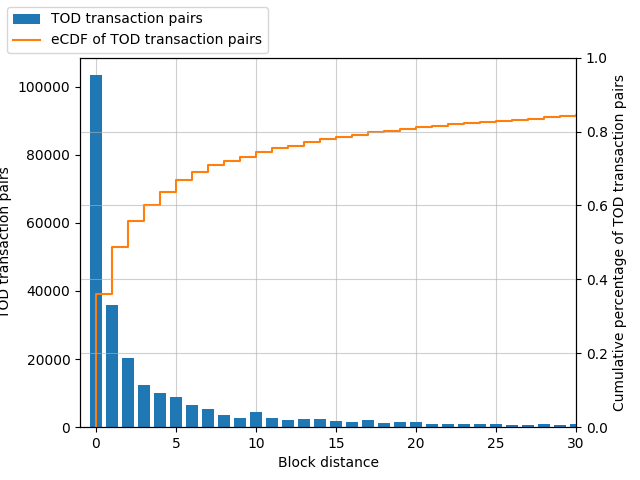
\includegraphics[width=0.8\textwidth]{tod_collisions_hist.png}
    \caption{The histogram and eCDF of the block distance for TOD candidates. The blue bars show how many TOD candidates have been found that are n blocks apart. The orange line shows the percentage of TOD candidates, that are at most n blocks apart.}
    \label{fig:tod_block_dist}
\end{figure}


\section{TOD candidate filtering}

Many of the TOD candidates we gain in the previous section are not relevant for our further analysis. To prevent unnecessary computation and distortion of our results, we filter them out.

We go through each filter in table \ref{tab:tod_candidate_filters} and filter out the TOD candidates that match the criteria.

\begin{table}[h]
    \begin{center}
        \begin{tabular}{ | l | l |  }
            \hline
            \thead{Filter name}      & \thead{Description of filter criteria}                                  \\ \hline
            Same-value collision     & \makecell[l]{Only take collisions where $T_A$ writes exactly the value, \\that is read or overwritten by $T_B$.} \\ \hline
            Nonce and code collision & Drop nonce and code collisions.                                         \\ \hline
            Block windows            & Drop transactions that are 25 or more blocks apart.                     \\ \hline
            Indirect dependency      & \makecell[l]{Drop TOD candidates with an indirect dependency.           \\e.g. if TOD candidates $(T_A, T_X)$ and $(T_X, T_B)$ exist.} \\ \hline
            Block producers          & Drop collisions on the block producer's balance.                        \\ \hline
            Same sender              & Drop if $T_A$ and $T_B$ are from the same sender.                       \\ \hline
            Recipient Ether transfer & Drop if $T_B$ does not execute code.                                    \\ \hline
        \end{tabular}
        \caption[TOD candidate filters]{TOD candidate filters sorted by usage order. When a filter describes the removal of collisions, the TOD candidates will be updated accordingly.}
        \label{tab:tod_candidate_filters}
    \end{center}
\end{table}
\subsection{Filters}

\subsubsection{Same-value collisions}

When we have many transactions that modify the same state, e.g. the balance of the same account, they will all have a write-write conflict with each other. The number of TOD candidates grows quadratic with the number of transactions modifying the same state. For instance, if 100 transactions modify the balance of address $a$, the first transaction would have a write-write conflict with all other 99 transactions, the second transaction with the remaining 98 transactions, etc., leading to a total of $\frac{n^2-n}{2} = 4950$ TOD candidates.

To reduce this growth of TOD candidates, we also require for a collision, that $T_A$ writes exactly the value that is read or overwritten by $T_B$. Formally, following must hold to pass this filter:

$$\forall K \in collisions(T_A, T_B)\colon poststate(\Delta_{T_A})(K) = prestate(\Delta_{T_B})(K)$$

With the example of 100 transactions modifying the balance of address $a$, when the first transaction sets to balance to 1234, it would only have a write-write conflict with transactions where the balance of $a$ was exactly 1234 before the execution. If all transactions wrote different balances, this would reduce the amount of TOD candidates to $n-1 = 99$.

\subsubsection{Nonce and Code collisions}

We showed in section \ref{sec:relevant-collisions}, that nonce and code collisions are not relevant for TOD attacks. Therefore, we ignore collisions for this state type.\todo{Implement this.}

\subsubsection{Block windows}

\todo{Mention, that this was also used by Frontrunner and Combatting paper.}

According to a study of 24 million transactions from 2019, the maximum observed transaction latency, from being pending to being included in a block, was below 200 seconds. If we combine this with the current block time, which is 12 seconds per block according to Etherscan \cite{etherscanio_ethereum_2024}, a transaction takes at most $\frac{200}{12} \approx 17$ blocks until a transaction is included in the blockchain, and an attacker can no longer frontrun it.

Therefore, if the blocks of two transactions are more than 17 blocks apart, a collision should not be because of a frontrunning attack. As the study is already 5 years old, we use a block window of 25 blocks instead, to account for a potential increase in latency since then.

Thus, we filter out all TOD candidates, where $T_A$ is in a block that is 25 or more blocks away from the block of $T_B$.

\subsubsection{Block producers}

In Ethereum, each transaction must pay a transaction fee to the block producer and thus modifies the block producer's balance. This would qualify each transaction pair in a block as a TOD candidate, as they all modify the balance of the block producer's address.

We exclude TOD candidates, where the only collision is the balance of any block producer.

\subsubsection{Indirect dependency}

As argued in section \ref{sec:weaknesses}, indirect dependencies can cause unexpected results in our analysis, therefore we will filter TOD candidates that have an indirect dependency.

We already have a model of all direct (potential) dependencies with the TOD candidates. We can build a transaction dependency graph $G = (V, E)$ with $V$ being all transactions and $E = \{ (T_A, T_B) \mid (T_A, T_B) \in \text{TOD candidates} \}$. We then filter out all TOD candidates $(T_A, T_B)$ where there exists a path $T_A, T_{X_1}, \dots, T_{X_n}, T_B$ with at least one intermediary node $T_{X_i}$.

Figure \ref{fig:tod_candidate_dependency} shows an example dependency graph, where transaction $A$ influences both $X$ and $B$ and $B$ is influenced by all other transactions. We would filter out the candidate $(A, B)$ as there is a path $A \rightarrow X \rightarrow B$, but keep $(X, B)$ and $(C, B)$.

\begin{figure}[h]
    \centering
    \begin{tikzpicture}
        \begin{scope}[
            >={Stealth[black]},
            every node/.style={circle,thick,draw},
            every edge/.style={draw=red,very thick}
            ]
            \node (A) at (3, 6) {A};
            \node (B) at (4, 3) {B};
            \node (C) at (5, 5) {C};
            \node (X) at (2, 4) {X};
            \path [->] (A) edge (B);
            \path [->] (A) edge (X);
            \path [->] (X) edge (B);
            \path [->] (C) edge (B);
        \end{scope}
    \end{tikzpicture}
    \caption{TOD candidate filters.}
    \label{fig:tod_candidate_dependency}
\end{figure}

\subsubsection{Same sender}

If the sender of both transactions is the same, the victim would have frontrun themselves.

To remove these TOD candidates, we use the information from the \verb|eth_getBlockByNumber| RPC method and compare the sender fields for $T_A$ and $T_B$.

\subsubsection{Recipient Ether transfer}

If a transaction sends Ether without execution code, it only depends on the balance of the EOA that signed the transaction. Other entities could only increase the balance of this EOA, by frontrunning the transaction, which has no adverse effects on the transaction.

When a transaction executes code, the trace will show this code access. Thus, we can exclude TOD candidates, where $T_B$ has no code access.

\subsection{Token filtering}

\todo{Consider filtering out TOD candidates related to tokens, e.g. by checking if a standardized token Log was emitted during transaction execution.}

\subsection{Deduplication}

\todo{Consider implementing deduplication, i.e. filtering out similar TOD candidates.}

\iffalse
    We want a diverse set of attacks for the benchmark, so we filter out similar attacks to the ones we already analyzed. For instance, it does not make sense to analyze 5000 attacks for the USDT Stablecoin, as these will mostly collide.

    If possible, we don't need the traces analyzer for deduplication. For instance, maybe we can get all the necessary information from the default RPC tracers.
    Alternatively, we could also download all necessary data, and then loop through the traces analyzer and only pick the relevant (deduplicated) potential attacks.

    Ideas, potentially a mixture of those:

    \begin{enumerate}
        \item only trace some attacks per contract
        \item only trace some attacks per function
        \item only trace some attacks per group of vulnerable contracts (as defined by analysis)
        \item only trace some attacks per contract/function skeletons
        \item similar to \cite{}, analyze at how many attacks per contract/function the number of found attacks saturate (based on the analysis result)
    \end{enumerate}
\fi

\chapter{Trace analysis}

% For instance, all EVM transactions in the same block read and write to the beneficiary account for gas payment, making all transactions interdependent by default.
% Is this the case? Do we see this in the prestate tracer?
% https://github.com/risechain/pevm

\section{Trace replaying}

\subsection{Algorithm}

Lets say, we have a transaction $T_A$ and a $T_B$, where $T_A$ occurred in block $Block_A$ and $T_B$ occurred in $Block_B$ (which may be equal to $Block_A$). Further, $T_A$ occurred before $T_B$, denoted as $T_A \rightarrow T_B$.

We want to replay following scenarios:

\begin{enumerate}
    \item actual: $T_A \rightarrow T_B$
    \item reverse: $T_B \rightarrow T_A$
\end{enumerate}

\subsubsection{Actual: $T_A \rightarrow T_B$}

For $T_A$: We start with $\sigma_{B_A}$, being the world state at the start of the block containing $T_A$. Then we set $\sigma = \sigma_{B_A} + \sum_{i=0}^{i=index(T_A)}\Delta_{T(B_B)_i}$ and execute $\sigma \xrightarrow{T_A} \sigma\prime$.

For $T_B$: We start with $\sigma_{B_B}$, being the world state at the start of the block containing $T_B$. Then we set $\sigma = \sigma_{B_B} + \sum_{i=0}^{i=index(T_B)}\Delta_{T(B_B)_i}$ and execute $\sigma \xrightarrow{T_B} \sigma\prime$.

\subsubsection{Reverse: $T_B \rightarrow T_A$}


For $T_B$: We start with $\sigma_{B_B}$, being the world state at the start of the block containing $T_B$. Then we set $\sigma = \sigma_{B_B} + (\sum_{i=0}^{i=index(T_B)}\Delta_{T(B_B)_i}) - \Delta_{T_A}$ and execute $\sigma \xrightarrow{T_B} \sigma\prime$.

For $T_A$: We start with $\sigma_{B_A}$, being the world state at the start of the block containing $T_A$. Then we set $\sigma = \sigma_{B_A} + (\sum_{i=0}^{i=index(T_A)}\Delta_{T(B_B)_i}) + \Delta_{T_B\prime}$ and execute $\sigma \xrightarrow{T_A} \sigma\prime$.

\section{Trace parsing}

Features:

\begin{enumerate}
    \item parses executed instructions with inputs and outputs
    \item handles internal transactions, including normal and exceptional halts
    \item tracks data origin for each byte of data, across calls and storages
    \item uses reference for DUPn instructions (so verification on one duplicate also verifies the other duplicate)
    \item outputs data flow graph, eg for source-sanitizers-sink analysis (and sanitizers could occur after sinks in Ethereum, because of reverts)
\end{enumerate}

Using traces instead of a full-fledged EVM allows:

\begin{enumerate}
    \item easier extension, as for instructions we only need to model their data flow
    \item interoperability with all nodes and other tools that produce traces
    \item automatic verification of the modelled data flows against the actual stack and memory
\end{enumerate}

\subsection{Data flow graph}

Horus and EVMTracer use a similar approach, by building a shadow state that contains the dependency information for each value.

We use a different approach, where our shadow state is directly used for computation. Furthermore, our approach is on byte level. Furthermore, our approach tracks data dependencies, rather than instruction step dependencies (and idk yet what exactly the dis-/advantages of that are).

\section{Attack categorization}

\section{Vulnerability localization}

\section{Attack labeling}

\chapter{TOD Attack results}

Findings of the TOD attack mining and analysis.

\chapter{Tool benchmarking}

\section{Systematic Literature Review}

\section{Setup}

\section{Result}



% %% intro.tex
%% Copyright (C) 2014-2023 by Thomas Auzinger <thomas@auzinger.name>
%
% This work may be distributed and/or modified under the
% conditions of the LaTeX Project Public License, either version 1.3
% of this license or (at your option) any later version.
% The latest version of this license is in
%   http://www.latex-project.org/lppl.txt
% and version 1.3 or later is part of all distributions of LaTeX
% version 2005/12/01 or later.
%
% This work has the LPPL maintenance status `maintained'.
%
% The Current Maintainer of this work is Thomas Auzinger.
%
% This work consists of the files vutinfth.dtx and vutinfth.ins
% and the derived file vutinfth.cls.
% This work also consists of the file intro.tex.


\newacronym{ctan}{CTAN}{Comprehensive TeX Archive Network}
\newacronym{faq}{FAQ}{Frequently Asked Questions}
\newacronym{pdf}{PDF}{Portable Document Format}
\newacronym{svn}{SVN}{Subversion}
\newacronym{wysiwyg}{WYSIWYG}{What You See Is What You Get}

\newglossaryentry{texteditor}
{
  name={editor},
  description={A text editor is a type of program used for editing plain text files.}
}

\chapter{Introduction to \LaTeX}

Since \LaTeX\ is widely used in academia and industry, there exists a plethora of freely accessible introductions to the language.
Reading through the guide at \url{https://en.wikibooks.org/wiki/LaTeX} serves as a comprehensive overview for most of the functionality and is highly recommended before starting with a thesis in \LaTeX.

\section{Installation}

A full \LaTeX\ distribution\index{distribution} consists not only of the binaries that convert the source files to the typeset documents, but also of a wide range of packages and their documentation.
Depending on the operating system, different implementations are available as shown in Table~\ref{tab:distrib}.
\textbf{Due to the large amount of packages that are in everyday use and due to their high interdependence, it is paramount to keep the installed distribution\index{distribution} up to date.}
Otherwise, obscure errors and tedious debugging ensue.

\begin{table}
  \centering
  \begin{tabular}{cccc}
    \toprule
    Distribution & Unix         & Windows      & MacOS        \\
    \midrule
    TeX Live     & \textbf{yes} & yes          & (yes)        \\
    MacTeX       & no           & no           & \textbf{yes} \\
    MikTeX       & (yes)        & \textbf{yes} & yes          \\
    \bottomrule
  \end{tabular}
  \caption{\TeX/\LaTeX\ distributions for different operating systems. Recomended choice in \textbf{bold}.}
  \label{tab:distrib} % \label has to be placed AFTER \caption to produce correct cross-references.
\end{table}

\section{Editors}

A multitude of \TeX\ \glspl{texteditor} are available differing in their editing models, their supported operating systems and their feature sets.
A comprehensive overview of \glspl{texteditor} can be found at the Wikipedia page  \url{https://en.wikipedia.org/wiki/Comparison_of_TeX_editors}.
TeXstudio (\url{http://texstudio.sourceforge.net/}) is recommended.
Most editors support a synchronization of the generated document and the \LaTeX\ source by \verb|Ctrl| clicking either on the source document or the generated document.

\section{Compilation}

Modern editors usually provide the compilation programs to generate \gls{pdf} documents and for most \LaTeX\ source files, this is sufficient.
More advanced \LaTeX\ functionality, such as glossaries and bibliographies, needs additional compilation steps, however.
It is also possible that errors in the compilation process invalidate intermediate files and force subsequent compilation runs to fail.
It is advisable to delete intermediate files (\verb|.aux|, \verb|.bbl|, etc.), if errors occur and persist.
All files that are not generated by the user are automatically regenerated.
To compile the current document, the steps as shown in Table~\ref{tab:compile} have to be taken.


\begin{table}
  \centering
  \begin{tabular}{rl}
    \toprule
    & Description \\
    \midrule
    1 & Scan for refs, toc/lof/lot/loa items and cites \\
    2 & Build the bibliography     \\
    3 & Link refs and build the toc/lof/lot/loa \\
    4 & Link the bibliography \\
    5 & Build the glossary \\
    6 & Build the acronyms \\
    7 & Build the index \\
    8 & Link the glossary, acronyms, and the index \\
    9 & Link the bookmarks \\
    \midrule
    & Command \\
    \midrule
    1 & \verb|pdflatex.exe  example| \\
    2 & \verb|bibtex.exe    example| \\
    3 & \verb|pdflatex.exe  example| \\
    4 & \verb|pdflatex.exe  example| \\
    5 & \verb|makeindex.exe -t example.glg -s example.ist| \\
      & \verb|              -o example.gls example.glo| \\
    6 & \verb|makeindex.exe -t example.alg -s example.ist| \\
      & \verb|              -o example.acr example.acn| \\
    7 & \verb|makeindex.exe -t example.ilg -o example.ind example.idx| \\
    8 & \verb|pdflatex.exe  example| \\
    9 & \verb|pdflatex.exe  example| \\
    \bottomrule
  \end{tabular}
  \caption{Compilation steps for this document. The following abbreviations were used: table of contents (toc), list of figures (lof), list of tables (lot), list of algorithms (loa).}
  \label{tab:compile} % \label has to be placed AFTER \caption to produce correct cross-references.
\end{table}


\section{Basic Functionality}

In this section, various examples are given of the fundamental building blocks used in a thesis.
Many \LaTeX\ commands have a rich set of options that can be supplied as optional arguments.
The documentation of each command should be consulted to get an impression of the full spectrum of its functionality.

\subsection{Floats}

Two main categories of page elements can be differentiated in the usual \LaTeX\ workflow: \textit{(i)} the main stream of text and \textit{(ii)} floating containers that are positioned at convenient positions throughout the document.
In most cases, tables, plots, and images are put into such containers since they are usually positioned at the top or bottom of pages.
These are realized by the two environments \verb|figure| and \verb|table|, which also provide functionality for cross-referencing (see Table~\ref{tab:intro} and Figure~\ref{fig:intro}) and the generation of corresponding entries in the list of figures and the list of tables.
Note that these environments solely act as containers and can be assigned arbitrary content.

\subsection{Tables}

A table in \LaTeX\ is created by using a \verb|tabular| environment or any of its extensions, e.g., \verb|tabularx|.
The commands \verb|\multirow| and \verb|\multicolumn| allow table elements to span multiple rows and columns.

\begin{table}[h] % placement specifier
  \centering
  \begin{tabular}{lll}
    \toprule
    \multicolumn{2}{c}{Position} \\
    \cmidrule{1-2} % partial horizontal rule
    Group & Abbrev & Name \\
    \midrule
    Goalkeeper & GK & Paul Robinson \\
    \midrule
    \multirow{4}{*}{Defenders} & LB & Lucus Radebe \\
                               & DC & Michael Duburry \\
                               & DC & Dominic Matteo \\
                               & RB & Didier Domi \\
    \midrule
    \multirow{3}{*}{Midfielders} & MC & David Batty \\
                                 & MC & Eirik Bakke \\
                                 & MC & Jody Morris \\
    \midrule
    Forward & FW & Jamie McMaster \\
    \midrule
    \multirow{2}{*}{Strikers} & ST & Alan Smith \\
                              & ST & Mark Viduka \\
    \bottomrule
  \end{tabular}
  \caption{Adapted example from the \LaTeX guide at \url{https://en.wikibooks.org/wiki/LaTeX/Tables}. This example uses rules specific to the \texttt{booktabs} package and employs the multi-row functionality of the \texttt{multirow} package.}
  \label{tab:intro} % \label has to be placed AFTER \caption to produce correct cross-references.
\end{table}

\subsection{Images}

An image is added to a document via the \verb|\includegraphics| command as shown in Figure~\ref{fig:intro}.
The \verb|\subcaption| command can be used to reference subfigures, such as Figure~\ref{fig:intro:full width} and~\ref{fig:intro:half width}.

\begin{figure}[h]
  \centering
  \begin{subfigure}[b]{0.45\columnwidth}
    \centering
    
\includegraphics[width=\textwidth]{TUWI-Logo-Code.png}
    \subcaption{The TU Wien Informatics logo at text width.}
    \label{fig:intro:full width}
  \end{subfigure}
  \begin{subfigure}[b]{0.45\columnwidth}
    \centering
    
\includegraphics[width=0.5\textwidth]{TUWI-Logo-Code.png}
    \subcaption{The TU Wien Informatics logo at half the text width.}
    \label{fig:intro:half width}
  \end{subfigure}
  \caption[Optional caption for the figure list (often used to abbreviate long captions)]{The header logo at different sizes.} % Remove the [...] argument if the original caption should be used in the figure list.
  \label{fig:intro} % \label has to be placed AFTER \caption (or \subcaption) to produce correct cross-references.
\end{figure}

\subsection{Mathematical Expressions}

One of the original motivation to create the \TeX\ system was the need for mathematical typesetting.
To this day, \LaTeX\ is the preferred system to write math-heavy documents and a wide variety of functions aids the author in this task.
A mathematical expression can be inserted inline as $\sum_{n=1}^{\infty} \frac{1}{n^2} = \frac{\pi^2}{6}$ outside of the text stream as \[ \sum_{n=1}^{\infty} \frac{1}{n^2} = \frac{\pi^2}{6} \] or as numbered equation with
\begin{equation}
\sum_{n=1}^{\infty} \frac{1}{n^2} = \frac{\pi^2}{6}.
\end{equation}

\subsection{Pseudo Code}

The presentation of algorithms can be achieved with various packages; the most popular are \verb|algorithmic|, \verb|algorithm2e|, \verb|algorithmicx|, or \verb|algpseudocode|.
An overview is given at \url{https://tex.stackexchange.com/questions/229355}.
An example of the use of the \verb|alogrithm2e| package is given with Algorithm~\ref{alg:gauss-seidel}.

\begin{algorithm}
  \SetKw{BreakFor}{break for}
  \KwIn{A scalar~$\epsilon$, a matrix $\mathbf{A} = (a_{ij})$, a vector $\vec{b}$, and an initial vector $\vec{x}^{(0)}$}
  \KwOut{$\vec{x}^{(n)}$ with $\mathbf{A} \vec{x}^{(n)} \approx \vec{b}$}
  \For{$k\leftarrow 1$ \KwTo maximum iterations}
  {
     \For{$i\leftarrow 1$ \KwTo $n$}
     {
        $x_i^{(k)} = \frac{1}{a_{ii}} \left(b_i-\sum_{j<i} a_{ij} x_j^{(k)} - \sum_{j>i} a_{ij} x_j^{(k-1)} \right)$\;
     }
     \If{$\lvert\vec{x}^{(k)}-\vec{x}^{(k-1)}\rvert < \epsilon$}
     {\BreakFor\;}
  }
  \Return{$\vec{x}^{(k)}$\;}
  \caption{Gauss-Seidel}
  \label{alg:gauss-seidel} % \label has to be placed AFTER \caption to produce correct cross-references.
\end{algorithm}

\section{Bibliography}

The referencing of prior work is a fundamental requirement of academic writing and well supported by \LaTeX.
The \textsc{Bib}\TeX\ reference management software is the most commonly used system for this purpose.
Using the \verb|\cite| command, it is possible to reference entries in a \verb|.bib| file out of the text stream, e.g., as~\cite{Turing1936}.
The generation of the formatted bibliography needs a separate execution of \verb|bibtex.exe| (see Table~\ref{tab:compile}).

\section{Table of Contents}

The table of contents is automatically built by successive runs of the compilation, e.g., of \verb|pdflatex.exe|.
The command \verb|\setsecnumdepth| allows the specification of the depth of the table of contents and additional entries can be added to the table of contents using \verb|\addcontentsline|.
The starred versions of the sectioning commands, i.e., \verb|\chapter*|, \verb|\section*|, etc., remove the corresponding entry from the table of contents.

\section{Acronyms / Glossary / Index}

The list of acronyms, the glossary, and the index need to be built with a separate execution of \verb|makeindex| (see Table~\ref{tab:compile}).
Acronyms have to be specified with \verb|\newacronym| while glossary entries use \verb|\newglossaryentry|.
Both are then used in the document content with one of the variants of \verb|\gls|, such as \verb|\Gls|, \verb|\glspl|, or \verb|\Glspl|.
Index items are simply generated by placing \verb|\index|\marg{entry} next to all the words that correspond to the index entry \meta{entry}.
Note that many enhancements exist for these functionalities and the documentation of the \verb|makeindex| and the \verb|glossaries| packages should be consulted.

\section{Tips}

Since \TeX\ and its successors do not employ a \gls{wysiwyg} editing scheme, several guidelines improve the readability of the source content:
\begin{itemize}
\item Each sentence in the source text should start with a new line.
      This helps not only the user navigation through the text, but also enables revision control systems (e.g. \gls{svn}, Git) to show the exact changes authored by different users.
      Paragraphs are separated by one (or more) empty lines.
\item Environments, which are defined by a matching pair of \verb|\begin{name}| and \verb|\end{name}|, can be indented by whitespace to show their hierarchical structure.
\item In most cases, the explicit use of whitespace (e.g. by adding \verb|\hspace{4em}| or \verb|\vspace{1.5cm}|) violates typographic guidelines and rules.
      Explicit formatting should only be employed as a last resort and, most likely, better ways to achieve the desired layout can be found by a quick web search.
\item The use of bold or italic text is generally not supported by typographic considerations and the semantically meaningful \verb|\emph{|\texttt{$\dots$}\verb|}| should be used.
\end{itemize}

The predominant application of the \LaTeX\ system is the generation of \gls{pdf} files via the \textsc{Pdf}\LaTeX\ binaries.
In the current version of \textsc{Pdf}\LaTeX, it is possible that absolute file paths and user account names are embedded in the final \gls{pdf} document.
While this poses only a minor security issue for all documents, it is highly problematic for double blind reviews.
The process shown in Table~\ref{tab:ps2pdf} can be employed to strip all private information from the final \gls{pdf} document.

\begin{table}[h]
  \centering
  \begin{tabular}{rl}
  \toprule
  & Command \\
  \midrule
  1 & Rename the \gls{pdf} document \verb|final.pdf| to \verb|final.ps|. \\
  2 & Execute the following command: \\
    & \verb|ps2pdf -dPDFSETTINGS#/prepress ^| \\
    & \verb| -dCompatibilityLevel#1.4 ^| \\
    & \verb| -dAutoFilterColorImages#false ^| \\
    & \verb| -dAutoFilterGrayImages#false ^| \\
    & \verb| -dColorImageFilter#/FlateEncode ^| \\
    & \verb| -dGrayImageFilter#/FlateEncode ^| \\
    & \verb| -dMonoImageFilter#/FlateEncode ^| \\
    & \verb| -dDownsampleColorImages#false ^| \\
    & \verb| -dDownsampleGrayImages#false ^| \\
    & \verb| final.ps final.pdf| \\
  \bottomrule
  \end{tabular}

  On Unix-based systems, replace \verb|#| with \verb|=| and \verb|^| with \verb|\|.
  \caption{Anonymization of \gls{pdf} documents.}
  \label{tab:ps2pdf}
\end{table}

\section{Resources}

\subsection{Useful Links}

In the following, a listing of useful web resources is given.
\begin{description}
\item[\url{https://en.wikibooks.org/wiki/LaTeX}] An extensive wiki-based guide to \LaTeX.
\item[\url{http://www.tex.ac.uk/faq}] A (huge) set of \gls{faq} about \TeX\ and \LaTeX.
\item[\url{https://tex.stackexchange.com/}] The definitive user forum for non-trivial \LaTeX-related questions and answers.
\end{description}

\subsection[Comprehensive TeX Archive Network]{\gls{ctan}}

The \gls{ctan} is the official repository for all \TeX\ related material.
It can be accessed via \url{https://www.ctan.org/} and hosts (among other things) a huge variety of packages that provide extended functionality for \TeX\ and its successors.
Note that most packages contain \gls{pdf} documentation that can be directly accessed via \gls{ctan}.

In the following, a short, non-exhaustive list of relevant \gls{ctan}-hosted packages is given together with their relative path.
\begin{description}[itemsep=0ex]
\item[\href{https://www.ctan.org/pkg/algorithm2e}{algorithm2e}] Functionality for writing pseudo code.
\item[\href{https://www.ctan.org/pkg/amsmath}{amsmath}] Enhanced functionality for typesetting mathematical expressions.
\item[\href{https://www.ctan.org/pkg/amsfonts}{amssymb}] Provides a multitude of mathematical symbols.
\item[\href{https://www.ctan.org/pkg/booktabs}{booktabs}] Improved typesetting of tables.
\item[\href{https://www.ctan.org/pkg/enumitem}{enumitem}] Control over the layout of lists (\verb|itemize|, \verb|enumerate|, \verb|description|).
\item[\href{https://www.ctan.org/pkg/fontenc}{fontenc}] Determines font encoding of the output.
\item[\href{https://www.ctan.org/pkg/glossaries}{glossaries}] Create glossaries and list of acronyms.
\item[\href{https://www.ctan.org/pkg/graphicx}{graphicx}] Insert images into the document.
\item[\href{https://www.ctan.org/pkg/inputenc}{inputenc}] Determines encoding of the input.
\item[\href{https://www.ctan.org/pkg/l2tabu}{l2tabu}] A description of bad practices when using \LaTeX.
\item[\href{https://www.ctan.org/pkg/mathtools}{mathtools}] Further extension of mathematical typesetting.
\item[\href{https://www.ctan.org/pkg/memoir}{memoir}] The document class on upon which the \verb|vutinfth| document class is based.
\item[\href{https://www.ctan.org/pkg/multirow}{multirow}] Allows table elements to span several rows.
\item[\href{https://www.ctan.org/pkg/pgfplots}{pgfplots}] Function plot drawings.
\item[\href{https://www.ctan.org/pkg/pgf}{pgf/TikZ}] Creating graphics inside \LaTeX\ documents.
\item[\href{https://www.ctan.org/pkg/subcaption}{subcaption}] Allows the use of subfigures and enables their referencing.
\item[\href{https://www.ctan.org/tex-archive/info/symbols/comprehensive/}{symbols/comprehensive}] A listing of around 5000 symbols that can be used with \LaTeX.
\item[\href{https://www.ctan.org/pkg/voss-mathmode}{voss-mathmode}] A comprehensive overview of typesetting mathematics in \LaTeX.
\item[\href{https://www.ctan.org/pkg/xcolor}{xcolor}] Allows the definition and use of colors.
\end{description} % A short introduction to LaTeX.

\backmatter

\begin{aitools}
    No generative AI tools where used in the process of researching and writing this thesis.
\end{aitools}

% Use an optional list of figures.
\listoffigures % Starred version, i.e., \listoffigures*, removes the toc entry.

% Use an optional list of tables.
\cleardoublepage % Start list of tables on the next empty right hand page.
\listoftables % Starred version, i.e., \listoftables*, removes the toc entry.

% Use an optional list of alogrithms.
\listofalgorithms
\addcontentsline{toc}{chapter}{List of Algorithms}

% Add an index.
\printindex

% Add a glossary.
\printglossaries

% Add a bibliography.
\bibliographystyle{alpha}
\bibliography{references}

\end{document}